\documentclass{standalone}
\usepackage{tikz}
\usepackage{amsmath,amssymb}
\usetikzlibrary{positioning}

\begin{document}
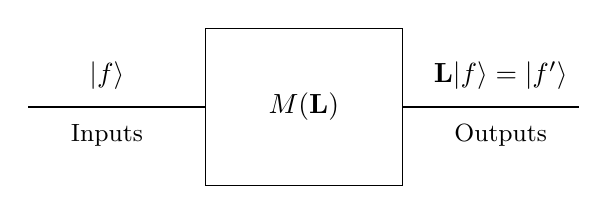
\begin{tikzpicture}
  % 定义样式
  \tikzset{
    block/.style={draw, rectangle, minimum width=2.5cm, minimum height=2cm},
    iotext/.style={font=\small},
    math/.style={font=\normalsize}
  }
  
  % 中央处理块
  \node[block] (process) at (0,0) {$M(\mathbf{L})$};
  
  % 输入侧
  \draw (-3.5,0) -- (process.west);
  \node[iotext, below] at (-2.5,-0.1) {Inputs};
  \node[math, above] at (-2.5,0.1) {$|f\rangle$};
  
  % 输出侧
  \draw (process.east) -- (3.5,0);
  \node[iotext, below] at (2.5,-0.1) {Outputs};
  \node[math, above] at (2.5,0.1) {$\mathbf{L}|f\rangle = |f'\rangle$};
\end{tikzpicture}
\end{document}